% Em TCC 2, colocar apenas Metodologia
\chapter{Metodologia proposta}
\label{cap:metodologia}

Este capítulo descreve a proposta de uma metodologia para o desenvolvimento de um chatbot para uso em disciplinas de nível de graduação, que poderá ser utilizado, em particular, na disciplina de Cálculo Numérico do Campus da UFC em Russas.

Na Seção \ref{sec:escopo}, é apresentado o escopo da futura aplicação do chatbot proposto. Em seguida, na Seção \ref{sec:escolha-tecnologias}, são pontuadas as escolhas das principais tecnologias que serão usadas no desenvolvimento da aplicação. Por fim, na Seção \ref{sec:funcionamento-chatbot}, é descrito como será o funcionamento do chatbot, tanto na interação com o aluno quanto com o professor.

\section{Escopo de uso}
\label{sec:escopo}

O intuito inicial do desenvolvimento desse chatbot é que ele seja aplicado em turmas futuras dos cursos de graduação da Universidade Federal do Ceará, no Campus de Russas. Devido ao seu escopo não ser limitado a uma disciplina ou área do conhecimento específica, ele pode ter seu uso expandido em demais cursos e em demais universidades. Entretanto, como caso de teste, será utilizada a disciplina de Cálculo Numérico, disciplina obrigatória para os cursos de Engenharia Civil, Engenharia Mecânica e Engenharia de Produção e optativa para o curso de Ciência da Computação neste campus.

\section{Escolha de tecnologias}
\label{sec:escolha-tecnologias}

A plataforma escolhida como meio de interação com o chatbot foi o Telegram, devido a ela ser uma plataforma popular atualmente, e a possuir uma API gratuita para o desenvolvimento de chatbots. O Telegram também é facilmente integrável com o Rasa, que será usado tanto para o processamento de linguagem natural das mensagens dos usuários, quanto para o gerenciamento do estado da conversa.

Além disso, a linguagem de programação escolhida para a implementação do projeto foi Python, pois ela é uma linguagem de fácil uso e flexível e, principalmente por conta do Rasa ser implementado majoritariamente em Python, o que permite uma fácil integração entre as duas tecnologias.

Por fim, para os dados que precisam ser persistidos durante a execução do sistema, será usado um banco de dados PostgreSQL, que será hospedado junto dos demais componentes do chatbot em um servidor virtual privado.

\section{Funcionamento do chatbot}
\label{sec:funcionamento-chatbot}

O funcionamento do chatbot será baseado em receber mensagens dos alunos solicitando recomendações de conteúdo sobre tópicos da disciplina. A partir disso, com base nos conteúdos disponíveis e no histórico de conversação com o aluno, será possível respondê-lo com recursos pertinentes à sua necessidade acadêmica, recursos estes que podem variar desde textos até mídias audiovisuais. Na Figura \ref{fig:chatbot-telegram-student}, é demonstrado um protótipo da interação de um aluno com o chatbot.

\begin{figure}[ht] 
   	\captionsetup{width=16cm}
	\Caption{\label{fig:chatbot-telegram-student} Protótipo de interação com o chatbot na visão do aluno}
	\UFCfig{}{
        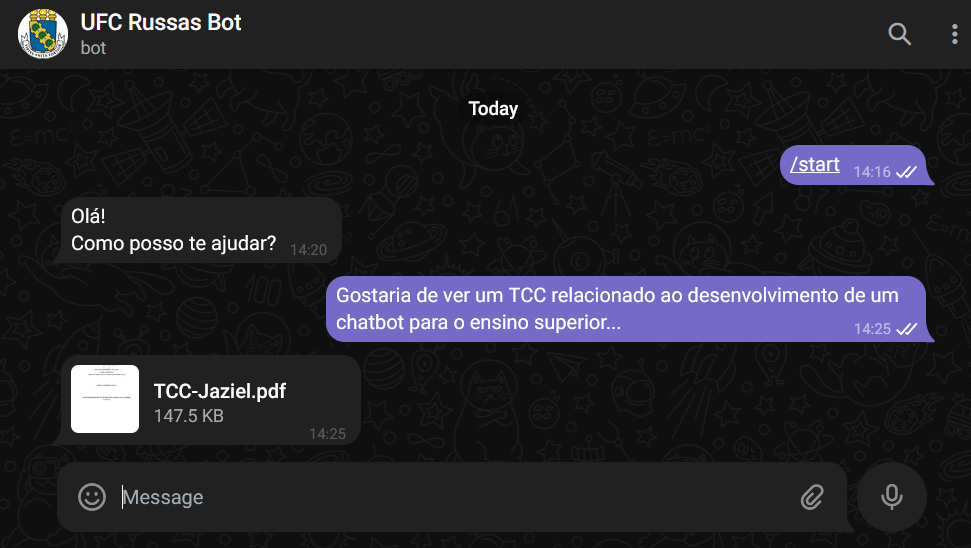
\includegraphics[width=16cm]{figuras/chatbot-telegram-student.png}
    }{
		\Fonte{Elaborado pelo autor}
	}
\end{figure}

Esses conteúdos recomendados pelo chatbot serão pré-cadastrados pelo professor da disciplina dentro da sua própria interface. Na Figura \ref{fig:chatbot-telegram-professor}, é apresentado um protótipo de como ocorrerá essa interação. É importante ressaltar que a API do Telegram não limita quais tipos de arquivos podem ser enviados, permitindo, assim, que o docente tenha uma ampla liberdade de inserir qualquer arquivo que desejar.

\begin{figure}[ht]
   	\captionsetup{width=16cm}
	\Caption{\label{fig:chatbot-telegram-professor} Protótipo de interação com o chatbot na visão do professor}
	\UFCfig{}{
        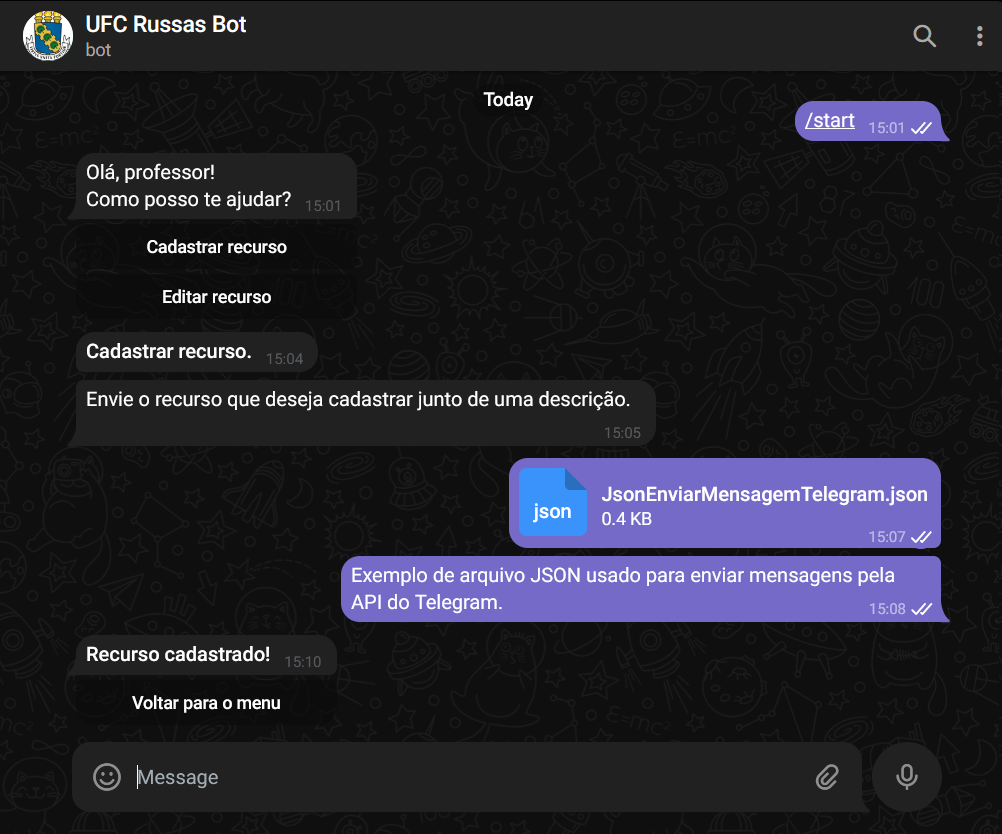
\includegraphics[width=16cm]{figuras/chatbot-telegram-professor.png}
    }{
		\Fonte{Elaborado pelo autor}
	}
\end{figure}

O acesso a diferentes funcionalidades dentro do chatbot será controlado por meio de perfis de acesso atrelados à conta do Telegram de cada usuário. Em um primeiro momento, os únicos perfis disponíveis serão o de docente e o de estudante. Caso não haja um perfil de acesso associado a uma determinada conta, será atribuído o perfil de acesso padrão, que é o de estudante.

\section{Considerações finais}
\label{sec:mp-consideracoes-finais}

Este capítulo descreveu a metodologia proposta para o desenvolvimento do chatbot que realize o objetivo geral desse trabalho. O próximo capítulo descreve sucintamente os resultados esperados com a aplicação desse chatbot.